% setwd(".")
% Sweave("script.rnw", syntax="SweaveSyntaxNoweb")
% pdflatex script.tex

% Modify for all subsequent chunks: \SweaveOpts{echo=FALSE}
% Or modify for that chunk only, put into <<>>=             @
% fig (FALSE), creates pdf / eps to be inserted from the plot command
% echo (TRUE), R input should be included
% label=xxx, text label for the code chunk, (also the first argument in options if not specified as label), use chunk reference operator <<>> to reference labels
% quiet, all progress messages are suppressed
% debug, input and output of code chunks copied to console
% eval (TRUE), code chunk is evaluated 
% keep.source (FALSE), when echoing, the original source is copied, else deparsed code is copied
% split (FALSE), write text output to seperate file for code chunk
% print (FALSE), wrap code in chunk in a print statement

\documentclass[a4paper]{article}
\usepackage{geometry}
%\usepackage{color}
\usepackage{framed}
\usepackage{setspace}
\usepackage{amsmath}
%\usepackage{hyperref}
\usepackage{times}
\usepackage{natbib}
%\usepackage{url}
\geometry{verbose,a4paper,tmargin=2cm,bmargin=1.5cm,lmargin=2cm,rmargin=3cm}
%\definecolor{shadecolor}{rgb}{0.9,0.9,0.9}
%\definecolor{darkblue}{rgb}{0,0,0.5}
\setlength{\parskip}{\medskipamount}
\setlength{\parindent}{0pt}
\onehalfspacing
%\hypersetup{colorlinks, urlcolor=darkblue}
\bibliographystyle{ecol_let}

\AtBeginDocument{
\DefineVerbatimEnvironment{Sinput}{Verbatim} {xleftmargin=2em,fontsize=
\footnotesize}
\DefineVerbatimEnvironment{Soutput}{Verbatim}{xleftmargin=2em,fontsize=
\footnotesize}
\DefineVerbatimEnvironment{Scode}{Verbatim}{xleftmargin=2em,fontsize=
\footnotesize}
}

% Title page
\usepackage{Sweave}
\begin{document}

\title{Using management strategy evaluation to design harvest control rules under decreasing survey effort}
\author{F. Scott <finlay.scott@cefas.co.uk\\
Cefas, Lowestoft, UK\\
C. Edwards <charles.edwards@imperial.ac.uk>\\
Imperial College London, Ascot, UK}
\date{March 2012}
\maketitle

%\begin{abstract}
%\end{abstract}


% Intro. What it does
\section{Introduction}

\section{The generic stock}

We start by generating a single stock using the $FLH$ generic life history generator. 
The parameters are given in Table~\ref{tab:genericStockParams} and the resulting reference points in Table~\ref{tab:genericRefPoints}.


% Table of parameters
\begin{table}
\centering
\begin{tabular}{|c|c|}
\hline
\multicolumn{2}{|c|}{Growth}\\
\hline
$L_{\infty}$ & 120     \\
$k$          & 0.192        \\
$maxage$     & 25\\
\hline
\multicolumn{2}{|c|}{Maturity}\\
\hline
$mat95$      & 6\\
\hline
\multicolumn{2}{|c|}{SRR}\\
\hline
$s$         & 0.75\\
$v$         & 1000\\
\hline
\end{tabular}
\caption{Parameters for generating the generic stock with $FLH$}
\label{tab:genericStockParams}
\end{table}

\begin{table}
\centering
\begin{tabular}{|c|c|}
\hline
\multicolumn{2}{|c|}{Reference points}\\
\hline
$MSY$       & 30.1924\\
$B^{MSY}$   & 380.989\\
$F^{MSY}$   & 0.0858183\\
\hline
\end{tabular}
\caption{Reference points for the generic stock with $FLH$}
\label{tab:genericRefPoints}
\end{table}

\begin{figure}
\centering
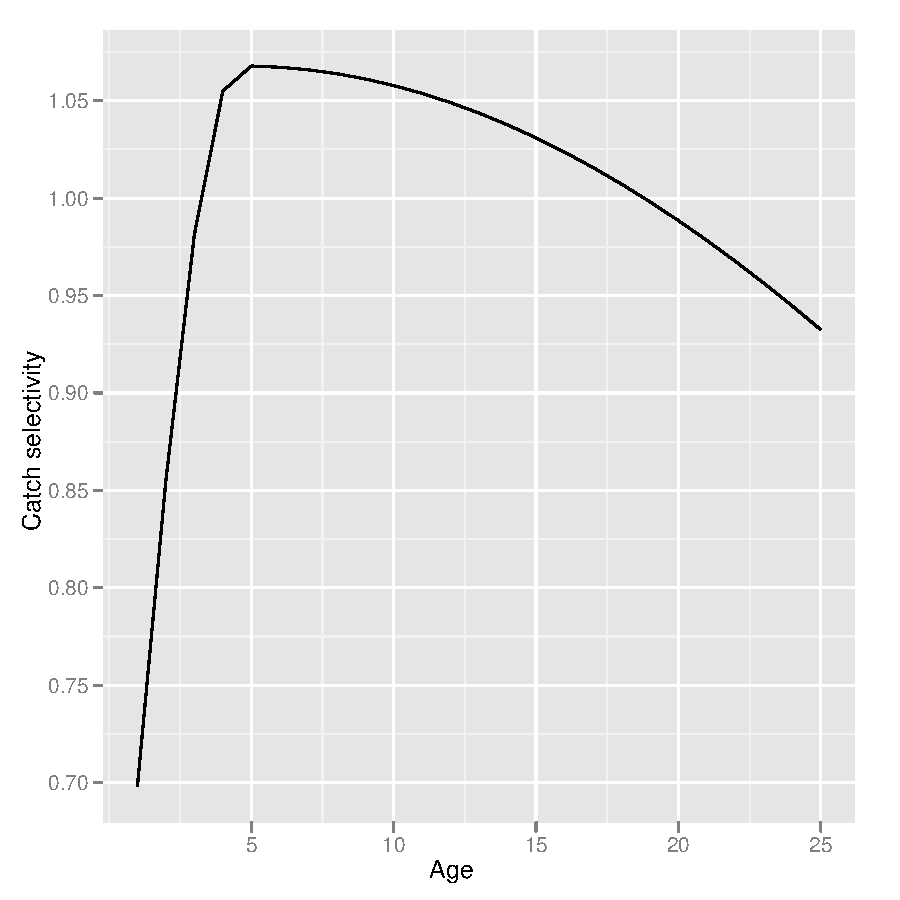
\includegraphics{script-genericSelectivityPlot}
\caption{Double normal catch selectivity curve for the generic stock with parameters $a1=0.5$, $sL=0.5$ and $sR=5$.}
\label{fig:generic_selectivity}
\end{figure}


%*******************************************************************************

\section{Historic stock trajectory}

\subsection{Historic fishing scenarios}

When \cite{Magnusson:2007} where investigating how information content
of the catch and index histories affected the assessment they used four different
scenarios of fishing mortality:

\begin{enumerate}
\item one-way trip, harvest rate gradually increases
\item no change, constant at a somewhat low harvest rate
\item good contrast, stock is fished down to less than half its initial size, then allowed to rebuild
\item rebuild only, stock begins at low abundance and is allowed to rebuild under low F
\end{enumerate}


We begin by looking at scenario 3 only: starting from 0, $F$ will increase to $2F^{MSY}$
before decreasing slightly over a period of 40 years. %We'll also multiply the $F$ value by lognormally distributed noise with a mean of 1 and a standard deviation of 0.1. 
You can see this in Figure~\ref{fig:Fscenario}. 

\begin{figure}
\centering
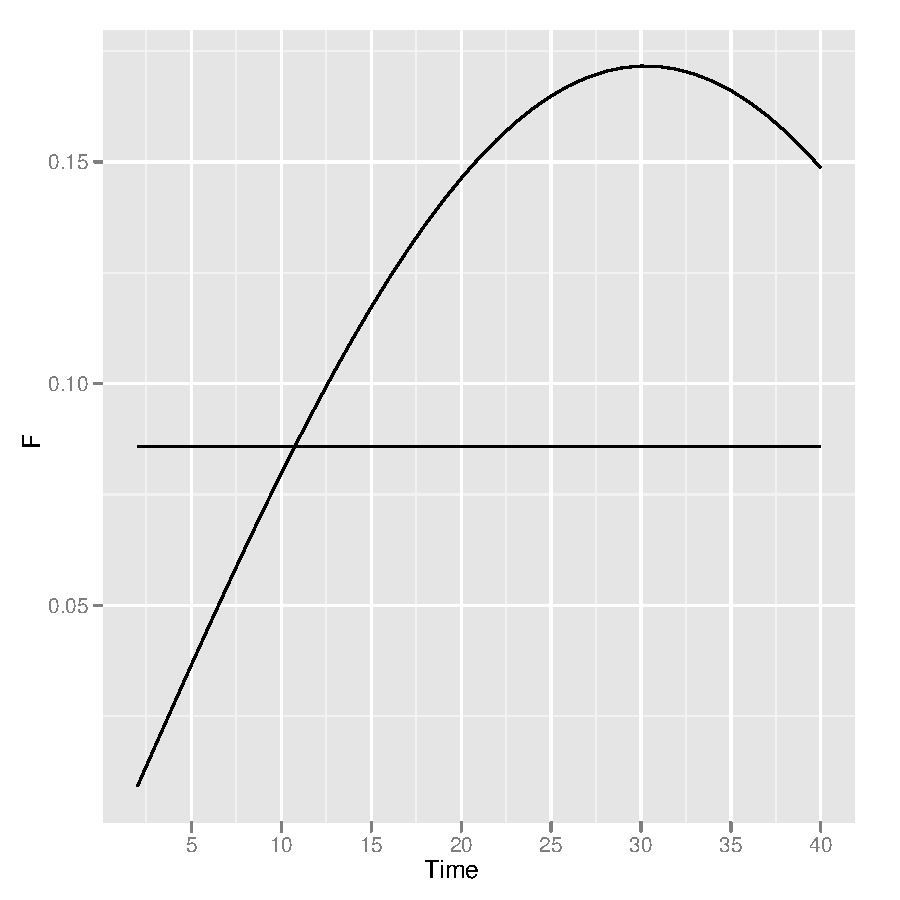
\includegraphics{script-F_plot1}
\caption{Fishing mortality scenario. $F$ increases from 0 to $2F^{MSY}$. The horizontal line is $F^{MSY}$.}
\label{fig:Fscenario}
\end{figure}

\subsection{Historic biomass trajectory}


Using the glory of $FLash$ we can now project the stock forward from time $t=0$ to $t=40$ under this fishing
scenario. %We'll put a small amount of lognormally distributed noise onto the recruitment with a mean of 1 and a standard deviation of 0.3.
To perform our projection we convert our generic stock (currently a $FLBRP$ object) into an $FLStock$ object,
define an $FLQuant$ containing the recruitment residuals, setup a control object and then project forward:

\begin{Schunk}
\begin{Sinput}
> stk1 <- as(gen1, "FLStock")
> stk1 <- window(stk1, end = maxt)
> ctrl_F1 <- fwdControl(data.frame(year = 2:maxt, quantity = "f", val = F1))
> sr_resid <- FLQuant(1, dimnames = list(age = 1, year = dimnames(stock.n(stk1))$year, iter = dimnames(stock.n(stk1))$iter))
> stk1 <- fwd(stk1, ctrl = ctrl_F1, sr = list(model = model(gen1), params = params(gen1)), sr.residuals = sr_resid)
\end{Sinput}
\end{Schunk}

The resulting stock object can be seen in Figure~\ref{fig:hist_proj}.

\begin{figure}
\centering
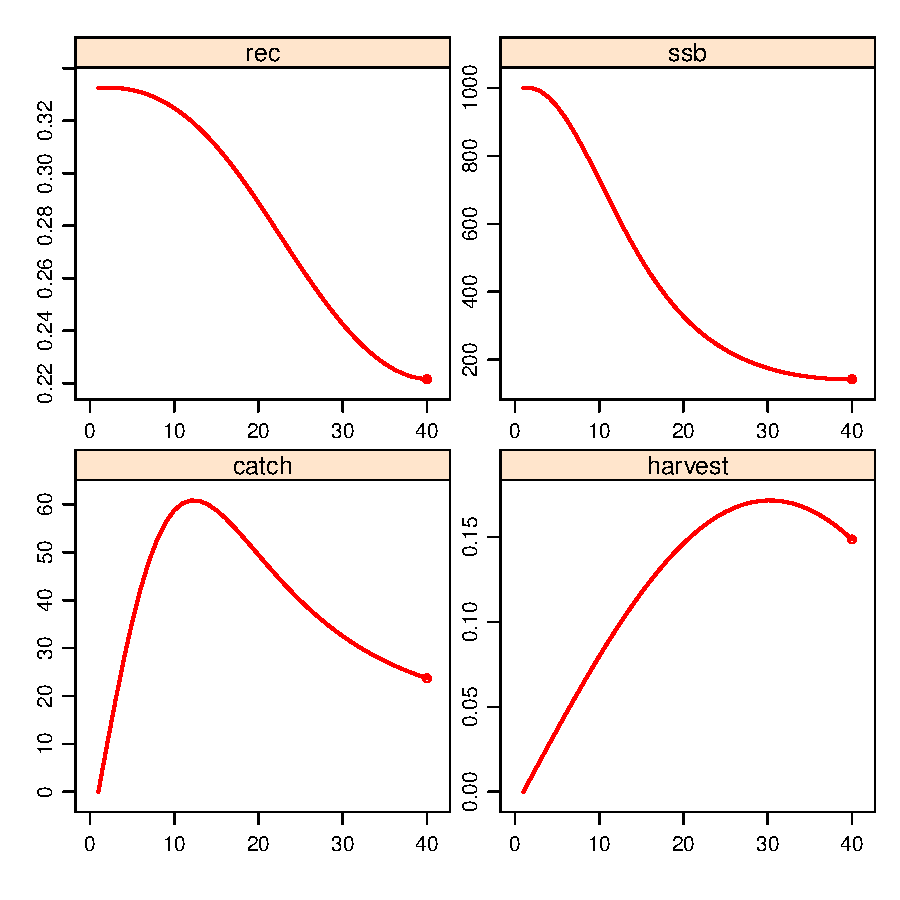
\includegraphics{script-hist_proj_plot}
\caption{Historic stock dynamics}
\label{fig:hist_proj}
\end{figure}


\section{Management scenarios}

We compared three different managment scenarios:
\begin{itemize}
\item perfect knowledge
\item model based control rule
\item empirical control rule
\end{itemize}

Management objectives are utilitarian, specified as both a target catch $C^{TAR}$ and catch rate $I^{TAR}$. 
Given that $MEY < MSY$, these are specified arbitarily as $C^{TAR} = 0.9 C^{MSY}$ and $I^{TAR} = 0.9 q B^{MSY}$ with $q=1e-4$.
Note that both targets are consistent with each other (i.e. it is feasible to achive both simultaneously).

The harvest conrol rule defines the catch per year
\[
C_{y+1} = \frac{C^{TAR}G(B_y)}{I^{TAR}}
\]
where $G(B_y)$ is our observation of the resource. For the scenarios listed above:
\begin{itemize}
\item $G(B_y) = qB_y$
\item $G(B_y) = \hat{q}\hat{B}_y$
\item $G(B_y) = I_y$
\end{itemize}

Since scenario 2 requires an estimation step, we predict that as survey effort declines performance of this control rule will deteriorate.
Specifically it will deteriorate at a faster rate than the control rule in scenario 3.

Performance was measured as the probability of $C>C^{TAR}$ and $I>I^{TAR}$ after a 20 year projection period. Managment scenarios will
be compared by a regression of performance against survey effort. 

\section{Management strategy projection}


\subsection{Getting the index data for the control rule}

We're going to assume the index comes from a
survey vessel so we need to set up a catch selectivity for the survey.
It's going to be sigmoid that is fully selected at age 4 (Figure~\ref{fig:survey_sel}).


\begin{figure}
\centering
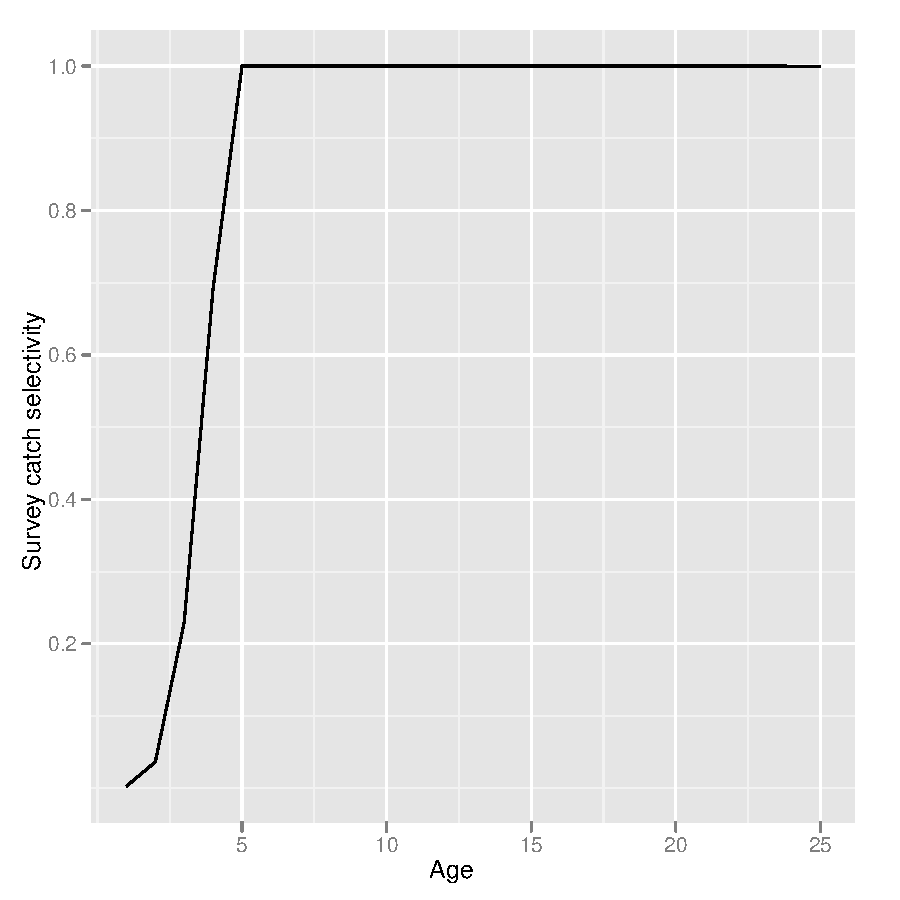
\includegraphics{script-survey_sel_plot}
\caption{The selectivity curve of the survey vessel}
\label{fig:survey_sel}
\end{figure}

We use empirical survey data to estimate the relationship between uncertainty in our catch rate index and the survey effort. Specifically, data
were extracted from the ICES International Bottom Trawl Survey (IBTS) database for the North Sea, and filtered for \textit{Gadus morhua} and the GOV gear type.
For each year from 1983 to 2011, bootstrap samples of individual trawls were taken, from which a mean catch rate in numbers per tow ($\hat{I}$) could
be estimated. The number of bootstrap samples represented the hypothesised survey effort. For each year and survey effort, we sampled 1000 values of $\hat{I}$
from the data, from which we obtained the coefficient of variation (Figure~\ref{fig:effCV}).

\begin{figure}
\centering
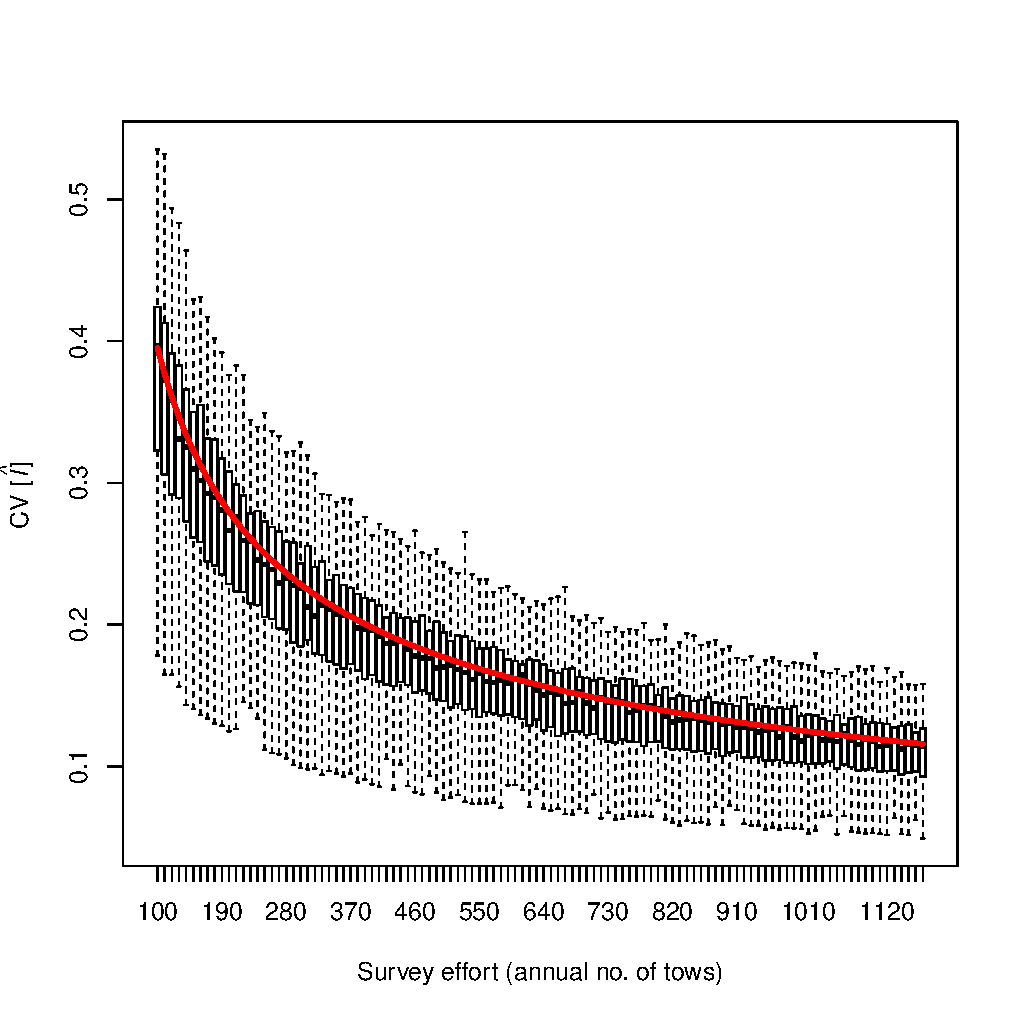
\includegraphics{../dat/effCV.pdf}
\caption{Estimated relationship between CV of the estimated catch rate and survey effort. Boxplots represent the variation across years.}
\label{fig:effCV}
\end{figure} 


We are going to generate historic survey data assuming the selectivity in Figure~\ref{fig:survey_sel}.
We now apply this selectivity to the population, and sum to get the index of abundance.
We assume that the survey takes place half way through the year
and we'll scale the abundance down by a 1000 (i.e. catchability $q=1e-4$). There is no observation error. The index
is asssumed to be perfectly known.

\begin{Schunk}
\begin{Sinput}
> index <- apply(sweep(stk2@stock.n * exp(-stk2@m/2) * stk2@stock.wt, 1:5, sselq, "*"), 2:6, sum) * 
+     1e-04
\end{Sinput}
\end{Schunk}

\section{Management simulation}

\subsection{Scenario 1: perfect knowledge}
\begin{Schunk}
\begin{Sinput}
> hcr <- function(catch, index, year) {
+     CTAR <- 0.9 * as.numeric(refpts(gen1)[, "yield"][4])
+     ITAR <- 0.9 * as.numeric(refpts(gen1)[, "biomass"][4]) * 1e-04
+     ILIM <- 0
+     GB <- as.numeric(quantSums(stock.n(stk2)[, year - 1] * stock.wt(stk2)[, year - 1] * catch.sel(gen1))) * 
+         1e-04
+     if (GB <= ILIM) {
+         TAC <- 0
+     }
+     else {
+         if (GB > ILIM & GB < ITAR) {
+             TAC <- (CTAR * (GB - ILIM))/(ITAR - ILIM)
+         }
+         else {
+             if (GB >= ITAR) {
+                 TAC <- (CTAR * GB)/ITAR
+             }
+         }
+     }
+     ctrl <- fwdControl(data.frame(year = year, val = TAC, quantity = "catch"))
+ }
\end{Sinput}
\end{Schunk}

\begin{figure}
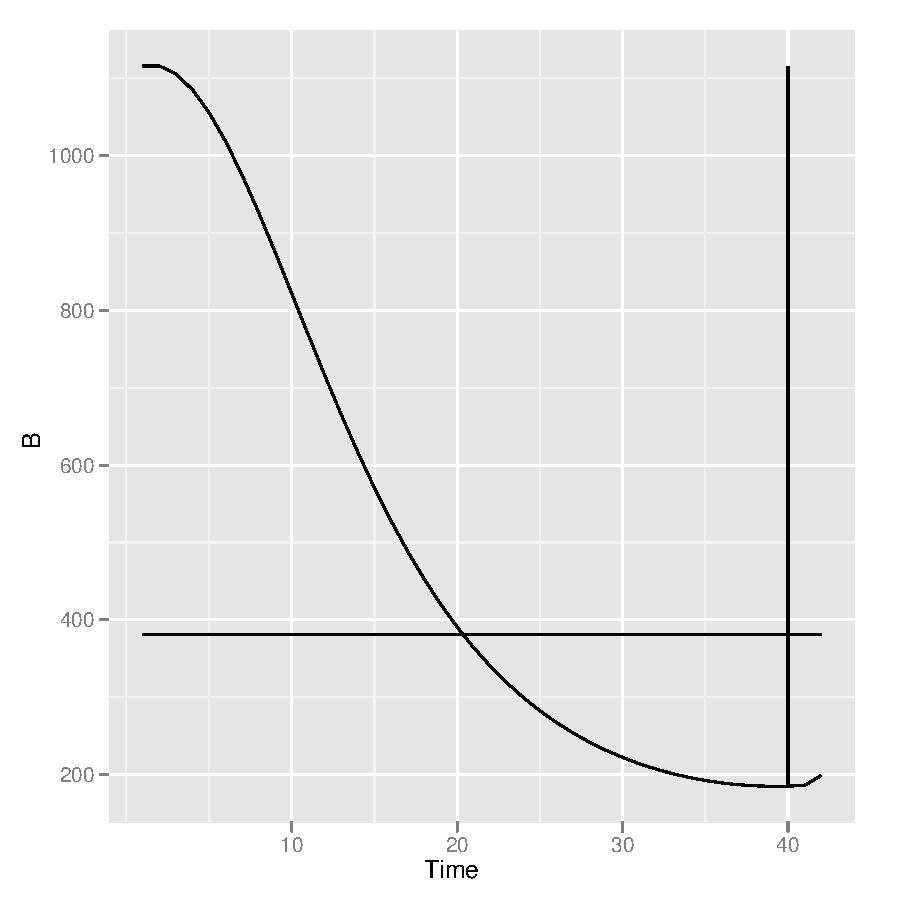
\includegraphics{script-hcr_plot_sc1}
\caption{The results of the projection}
\label{fig:hcr_proj_biomass}
\end{figure}

\subsection{Scenario 3: empirical control rule}
\begin{Schunk}
\begin{Sinput}
> hcr <- function(catch, index, year) {
+     CTAR <- 0.9 * as.numeric(refpts(gen1)[, "yield"][4])
+     ITAR <- 0.9 * as.numeric(refpts(gen1)[, "biomass"][4]) * 1e-04
+     ILIM <- 0
+     GB <- as.numeric(index[, year - 1])
+     if (GB <= ILIM) {
+         TAC <- 0
+     }
+     else {
+         if (GB > ILIM & GB < ITAR) {
+             TAC <- (CTAR * (GB - ILIM))/(ITAR - ILIM)
+         }
+         else {
+             if (GB >= ITAR) {
+                 TAC <- (CTAR * GB)/ITAR
+             }
+         }
+     }
+     ctrl <- fwdControl(data.frame(year = year, val = TAC, quantity = "catch"))
+ }
\end{Sinput}
\end{Schunk}

\begin{figure}
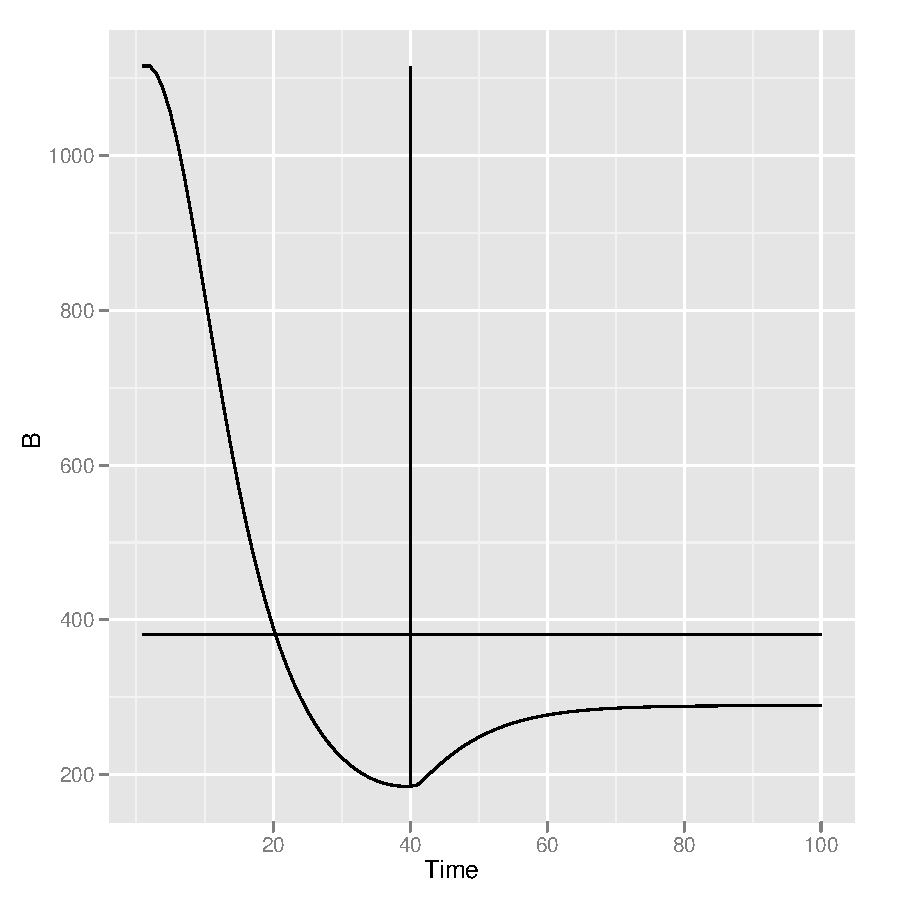
\includegraphics{script-hcr_plot_sc3}
\caption{The results of the projection}
\label{fig:hcr_proj_biomass}
\end{figure}



\newpage
\bibliography{lib}

R
FLR
Sweave
Polacheck


\end{document}

